\documentclass[12pt]{article}

% Pakete
\usepackage{ngerman,a4}
\usepackage[latin1]{inputenc}
\usepackage{makeidx}
\usepackage{exscale,icomma}
\usepackage{amsbsy,amscd,amsfonts,amsmath,amssymb,amstext,amsthm,amsxtra}
\usepackage{moreverb}
\usepackage{algorithm}
\usepackage{algorithmic}

\usepackage{graphicx}

% L�ngen festlegen
%\setlength{\parindent}{0pt}
\setlength{\unitlength}{1cm}

% Kurzbefehle: Aufz�hlungen
\newcommand{\letter}{\renewcommand{\labelenumi}{\alph{enumi})}}

% Kurzbefehle: Symbole
\newcommand{\�}{\text{ }} \renewcommand{\sp}{\hspace{0.5cm}}
\newcommand{\nat}{\mathbb{N}} \newcommand{\ganz}{\mathbb{Z}} \newcommand{\rat}{\mathbb{Q}} \newcommand{\real}{\mathbb{R}} \newcommand{\comp}{\mathbb{C}}
\newcommand{\pot}{\mathcal{P}} \newcommand{\loes}{\mathbb{L}}
\newcommand{\bigO}{\mathcal{O}} \newcommand{\bigP}{\mathsf{P}}  \newcommand{\bigNP}{\mathsf{NP}}
\newcommand{\vpunkt}{\enspace\vdots}

% Kurzbefehle: Erkl�rung in Formeln
\newcommand{\erklaerLU}[2]{\underset{\parbox[l]{0.2cm}{\makebox[10cm][l]{\scriptsize $#2$}}}{\underbrace{#1}}}
\newcommand{\erklaerLO}[2]{\overset{\parbox[l]{0.2cm}{\makebox[10cm][l]{\scriptsize $#2$}}}{\overbrace{#1}}}
\newcommand{\erklaerCU}[2]{\underset{\makebox[0cm][c]{\scriptsize $#2$}}{\underbrace{#1}}}
\newcommand{\erklaerCO}[2]{\overset{\makebox[0cm][c]{\scriptsize $#2$}}{\overbrace{#1}}}

\begin{document}

% Titel
\title{Algorithmen f�r Fortgeschrittene}
\author{Jan Sebastian Siwy \and Martin Spickermann}
\date{2. Vorlesung vom 15. April 2004}
\maketitle

% Inhalt
\paragraph{Nachtrag:} Bildung des Restnetzes aus der letzten Vorlesung.
\begin{center}
    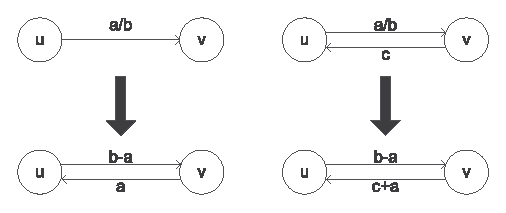
\includegraphics{2004-04-15-fluss-ford-fulkerson/grafiken/Grafik1}
\end{center}
Kanten mit der Kapazit�t $0$ k�nnen weggelassen werden.

\paragraph{Korollar:} Der Wert jedes Flusses im Netz $G$ ist durch die minimale Kapazit�t aller denkbarer Schnitte nach oben beschr�nkt, denn
$$ f(S, T) \leq c(s, t). $$
Im Beispiel kann der Fluss nicht gr��er sein als $23$ (Schnittverlauf laut Skizze):
\begin{center}
    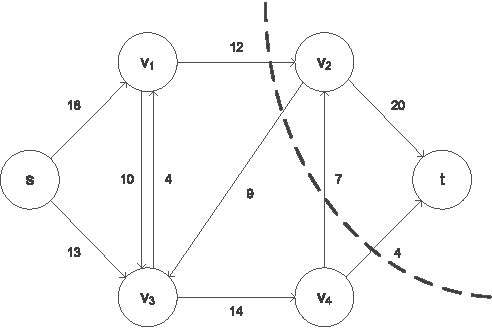
\includegraphics{2004-04-15-fluss-ford-fulkerson/grafiken/Grafik2}
\end{center} \pagebreak[3]

\paragraph{Satz 1:} Sei $f$ Fluss im Netz $G_f$, dann sind folgende Aussagen �quivalent:
\begin{enumerate}
    \item $f$ ist maximal.
    \item Es gibt keine augmentierenden Wege bzgl. $G, c, f$.
    \item Es gibt einen Schnitt $S, T$ mit $|f| = c(S, T)$. \par
    (Bemerkung: Dieser Schnitt hat minimale Kapazit�t.)
\end{enumerate}

\paragraph{Beweis:}
\begin{itemize}
    \item $1 \Rightarrow 2$: \par
    trivial
    \item $2 \Rightarrow 3$: \par
    Es gibt in $G$ keinen augmentierenden Weg, d.h. in $G_f$ gibt es keinen Weg von $s$ nach $t$. \par
    Sei $S = \{ v \in V \; | \; \exists \text{ Weg von $s$ nach $v$ in $G_f$} \}$ und $T = V \backslash S$. \par
    Betrachte Schnitt $S, T$, bei dem $f(u, v) = c(u, v)$ f�r alle $u \in S$ und $v \in T$. \par
    Daraus folgt:
    \begin{align*}
        |f| &= f(S, T) \tag{nach Lemma 2} \\
            &= c(S, T)
    \end{align*}
    \item $3 \Rightarrow 1$: \par
    Nach dem Korollar gilt $|f| \leq c(S, T)$ f�r alle Fl�sse und Schnitte, also auch f�r diesen. \par
    Da $|f| = c(S, T)$ gilt, ist $f$ maximal.
\end{itemize} \hfill $\Box$

\paragraph{Ford-Fulkerson-Algorithmus (Schema):}

\begin{algorithmic}[1]
    \STATE Initialisiere den Fluss $f$ auf $0$.
    \WHILE {$\exists$ augmentierender Weg $p$ von $s$ nach $t$ im Restnetz $G_f$}
    \STATE $\forall$ Kante $e \in p$ erh�he den Fluss $f$ um die Kapazit�t $c_f(p)$ dieses Weges, wobei $c_f(p) = \min c_f(e)$
    \ENDWHILE
\end{algorithmic} \pagebreak[3]

In unserem Beispiel:
\begin{itemize}
    \item Initialisierung:
    \begin{center}
        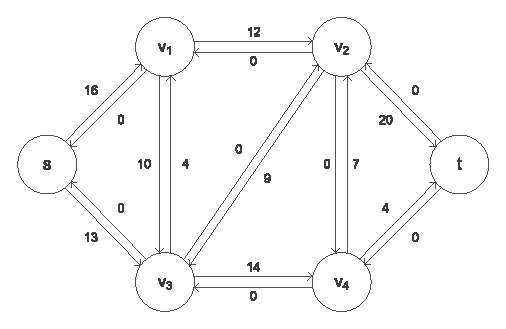
\includegraphics{2004-04-15-fluss-ford-fulkerson/grafiken/Grafik3}
    \end{center}
    \item Schritt 1 (Weg �ber $s, v_1, v_3, v_4, v_2, t$ mit Minimum $7$):
    \begin{center}
        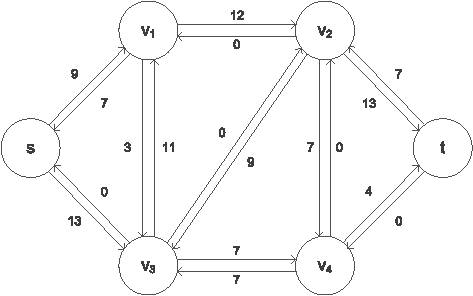
\includegraphics{2004-04-15-fluss-ford-fulkerson/grafiken/Grafik4}
    \end{center}
    \item Schritt 2 (Weg �ber $s, v_1, v_2, t$ mit Minimum $9$):
    \begin{center}
        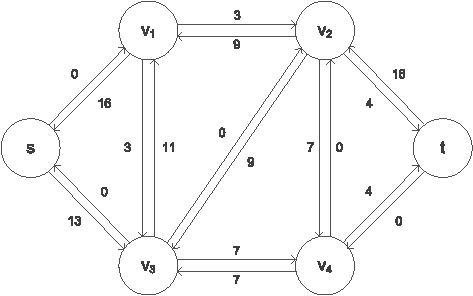
\includegraphics{2004-04-15-fluss-ford-fulkerson/grafiken/Grafik5}
    \end{center} \pagebreak[3]
    \item Schritt 3 (Weg �ber $s, v_3, v_4, t$ mit Minimum $4$):
    \begin{center}
        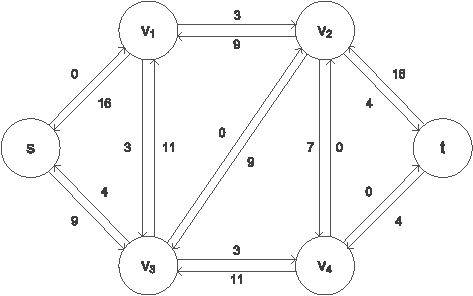
\includegraphics{2004-04-15-fluss-ford-fulkerson/grafiken/Grafik6}
    \end{center}
    \item Schritt 4 (Weg �ber $s, v_3, v_1, v_2, t$ mit Minimum $3$):
    \begin{center}
        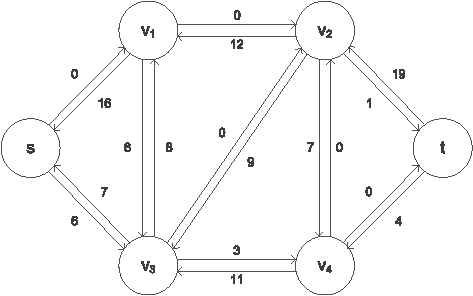
\includegraphics{2004-04-15-fluss-ford-fulkerson/grafiken/Grafik7}
    \end{center}
    \item L�sung:
    \begin{center}
        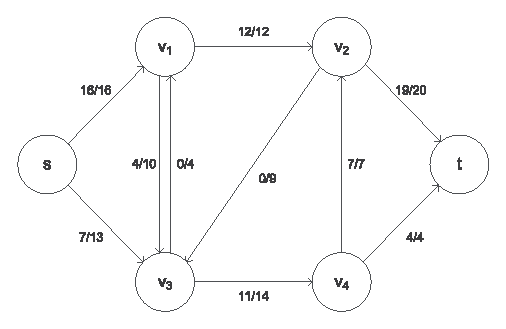
\includegraphics{2004-04-15-fluss-ford-fulkerson/grafiken/Grafik8}
    \end{center}
\end{itemize} \pagebreak[3]

\paragraph{Einzelheiten des Algorithmus:}
\begin{itemize}
    \item Schritt 1: \par
    Variable f�r Fluss $f$ definieren und diese auf $0$ setzen.
    \item Schritt 2: \par
    Finden eines Weges. Konstruiere dazu als Datenstruktur einen Graphen $G'$:
    $$ G' = (V, E') \sp \text{mit} \sp E' = E \cup \{ (u, v) \; | \; (v, u) \in E \} $$
    Jedes Restnetz ist Teilgraph von $G'$. Kanten mit Rest $0$ k�nnen ignoriert werden.
    \item Schritt 3: \par
    Konstruktion bzw. Aktualisierung des Restnetzes.
\end{itemize}

\paragraph{Laufzeitanalyse:}
\begin{itemize}
    \item Schritt 1: \par
    Kostet $\bigO(|E|)$.
    \item Schritt 2: \par
    Kostet $\bigO(|E|)$ mit Breiten- oder Tiefensuche pro Durchlauf.
    \item Schritt 3: \par
    Kostet $\bigO(|E|)$ pro Durchlauf. \par
    Jede Kante auf $p$ und die Gegenkante muss aktualisiert werden.
\end{itemize}
 Wie viele Durchl�ufe ben�tigt nun der Algorithmus insgesamt?
 \begin{itemize}
    \item Bei jedem Durchlauf wird der Fluss erh�ht.
    \item Wenn wir annehmen, dass die Kapazit�ten ganze Zahlen sind, erh�ht sich der Fluss um mindestens $1$ je Durchgang.
 \end{itemize}
 Wenn $f^*$ der maximale Fluss ist, so gibt es h�chstens $|f^*|$ Durchl�ufe. Die Laufzeit des Ford-Fulkerson-Algorithmus ist also $\bigO(|E| \cdot |f^*|)$.

 \paragraph{Bemerkungen durch Laufzeitanalyse:} Diese Aussage zur Laufzeit ist unbefriedigend, weil
 \begin{itemize}
    \item wir angenommen haben, dass die Kapazit�ten ganze Zahlen sind und
    \item der maximale Fluss $|f^*|$ exponentiell zur Eingabegr��e sein kann.
 \end{itemize}
Der maximale Fluss $|f^*|$ ist tats�chlich m�glich!
\begin{center}
    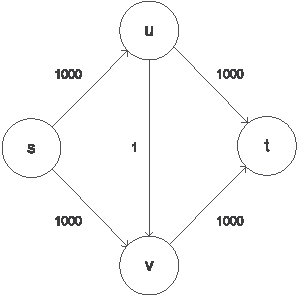
\includegraphics{2004-04-15-fluss-ford-fulkerson/grafiken/Grafik9}
\end{center}
Es werden 2000 Durchl�ufe erreicht, wenn abwechselnd die Pfade $s, u, v, t$ und $s, v, u, t$ gew�hlt werden.

\paragraph{Edmond-Karp-Algorithmus:} Dieser findet immer den k�rzesten Weg durch Breitensuche in Schritt 2.

\paragraph{Lemma 3:} Sei $\delta_f(u, v)$ der Abstand $u, v \in V$ im Restnetz $G_f$. \par
Beim Edmond-Karp-Algorithmus gilt f�r alle Knoten $v \in V \backslash \{ s, t \}$, dass in jedem augmentierendem Schritt der Abstand $\delta_f(u, v)$ monoton w�chst.

\paragraph{Beweis:} Angenommen das Lemma gilt nicht, d.h. es existieren ein augmentierender Schritt und ein Knoten $v$, so dass $\delta_{f'}(s, v) < \delta_f(s, v)$ gilt mit $f$ Fluss vor und $f'$ Fluss nach dem augmentierendem Schritt. \par
O.b.d.A. sei $v$ der Knoten mit der Eigenschaft, dass der Abstand $\delta_f(s, v)$ minimal ist. Der k�rzeste Weg von $s$ nach $v$ in $G_{f'}$ sei $p'$. Der Knoten $u$ sei der vorletzte Knoten auf diesem Weg $p'$.
\begin{center}
    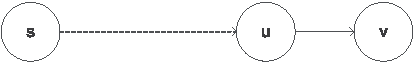
\includegraphics{2004-04-15-fluss-ford-fulkerson/grafiken/Grafik10}
\end{center} \pagebreak[3]
Wegen der Minimalit�t von $v$ gilt $\delta_{f'}(s, v) \geq \delta_f(s, u)$. Betrachte den Fluss $f(u, v)$ vor dem augmentierenden Schritt:
\begin{itemize}
    \item Fall 1: $f(u, v) < c(u, v)$, d.h. $(u, v)$ ist eine Kante in $G_f$.
    \begin{align*}
        \delta_f(s, v) &\leq \delta_f(s, u) + 1 \\
                       &\leq \delta_{f'}(s, u) + 1 \\
                       &= \delta_{f'}(s, v) \tag{Widerspruch!}
    \end{align*}
    \item Fall 2: $f(u, v) = c(u, v)$, d.h. $(u, v)$ ist keine Kante in $G_f$. \par
    Damit muss der augmentierende Weg $p$ die Kante $(u, v)$ enthalten haben.
    \begin{center}
        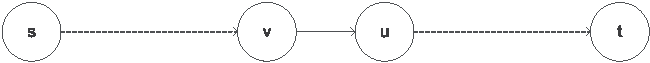
\includegraphics{2004-04-15-fluss-ford-fulkerson/grafiken/Grafik11}
    \end{center}
    \begin{align*}
        \delta_f(s, v) &= \delta_f(s, u) - 1 \\
                       &\leq \delta_{f'}(s, u) - 1 \\
                       &= \delta_{f'}(s, v) - 2 \\
                       &< \delta_{f'}(s, v) \tag{Widerspruch!}
    \end{align*} \hfill $\Box$
\end{itemize}




\end{document}
